\chapter{Formatowanie}

Styl formatowania został określony w pliku \verb|thesis.cls|, stąd nie ma potrzeby ręcznego formatowania kolejnych fragmentów pracy. Numerowanie wzorów, tabel, rysunków i rozdziałów, generowanie bibliografii oraz spisu treści odbywa się automatycznie. Zmiana danych strony tytułowej odbywa się na drodze edycji pliku \verb|thesis.tex|. Zadanie autora sprowadza się zatem jedynie do wprowadzenia treści pracy.

\section{Wklejanie rysunków}

Standardowo rysunki wklejane są do dokumentu pomiędzy akapitami. Przykład takiego rozwiązania przedstawia rysunek~\ref{fig:rys_1}. Rysunki można wstawiać również w ten sposób, że są one otoczone tekstem, stosując bibliotekę \verb|wrapfigure|. Nie zaleca się jednak takiego rozwiązania, chyba że rysunek jest bardzo mały, a jego opis zwięzły. Numerowanie rysunków jest automatyczne, a odwoływanie się do nich możliwe jest stosując \verb|\ref{nazwa_rysunku}|, przy czym nazwa ta wskazywana jest podczas wstawiania rysunku.

\begin{figure}[htb!]
\centering
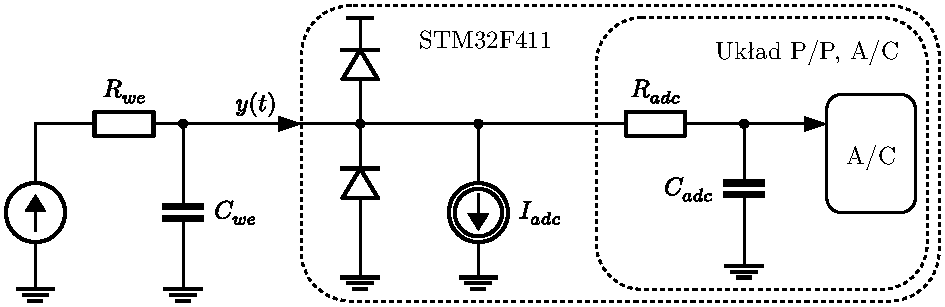
\includegraphics{schemat_adc}
\makecaption{fig:rys_1}{Przykładowy rysunek (źródło: \url{https://github.com/Kuszki/Phd})}
\end{figure}

Rysunki należy sporządzać w formacie wektorowym (np. stosując program \verb|LibreOffice|). Wykresy generowane przez programy \verb|GNU Octave| oraz \verb|MATLAB| mogą być eksportowane do formatu \verb|SVG|. Natywne w \LaTeX{} obsługiwane są obrazy w formacie \verb|PDF|. Wszystkie pliki z rozszerzeniami \verb|.odg| oraz \verb|.svg|, znajdujące się w folderze \verb|obrazki|, będą jednak automatycznie skonwertowane do tego formatu podczas uruchamiania skryptu \verb|build.sh|. Należy unikać stosowania obrazków w formacie rastrowym (np. \verb|.jpeg| lub \verb|.png|), chyba że stanowią one zdjęcie lub nie ma możliwości sporządzenia rysunku w formacie wektorowym.

\section{Wklejanie tabel}

Sporządzanie tabel w \LaTeX{} nie jest przyjemne i wymaga odrobinę wprawy. Rozwiązanie to odwdzięcza się jednak jednolitym wyglądem oraz sporą możliwością automatyzacji formatowania danych. W przypadku tabel z wynikami pomiarów bardzo dobrym pomysłem jest stosowanie biblioteki \verb|siunitx|. Biblioteka ta zapewnia czytelne wyrównanie wartości liczbowych, a także uniezależnia dane od formatu ich wyświetlania (istotne np. gdy skopiowane wyniki posiadają kropkę jako separator dziesiętny, a lokalny format wymaga przecinka). Tabele~\ref{tab:tab_1} oraz~\ref{tab:tab_2} stanowią przykłady, gdzie zamieszczono wyniki eksperymentów.

\begin{table}[htb!]
\centering
\makecaption{tab:tab_1}{Przykład tabeli, gdzie kolejne symbole oznaczają rozkład: $(n)$~normalny, $(u)$~jednostajny, $(t)$~trójkątny, $(d)$~dwumodalny (źródło: \url{https://github.com/Kuszki/Phd})}
\begin{tabular}[c]{| c *{4}{|S[table-format = 1.4]} |} \hline
$s_{a,b}$ & \textbf{$n$} & \textbf{$u$} & \textbf{$t$} & \textbf{$d$} \\ \hline
$n$       & 0.0000       & 0.1561       & 0.0250       & 0.2988       \\ \hline
$u$       & 0.1561       & 0.3356       & 0.1773       & 0.5337       \\ \hline
$t$       & 0.0250       & 0.1773       & 0.0419       & 0.3504       \\ \hline
$d$       & 0.2988       & 0.5337       & 0.3504       & 0.7136       \\ \hline
\end{tabular}
\end{table}

\begin{table}[htb!]
\centering
\makecaption{tab:tab_2}{Inna przykładowa tabela z wynikami (źródło: \url{https://github.com/Kuszki/Phd})}
\begin{tabular}[c]{| c *{5}{|S[table-format = 2.2]} *{4}{|S[table-format = +1.2]} |} \hline
\multirow{2}{*}{\textbf{Wielkość}} & \multicolumn{5}{c|}{\textbf{Niepewność, mV}} & \multicolumn{4}{c|}{\textbf{Błąd, \%}} \\ \cline{2-10}
& $U_{a}$ & $U_{b}$ & $U_{c}$ & $U_{d}$ & $U_{s}$ & $\delta_{a}$ & $\delta_{b}$ & $\delta_{c}$ & $\delta_{d}$ \\ \hline
$S_{2,0}$ & 75.01 & 74.00 & 74.10 & 77.32 & 72.87 & +2.94 & +1.55 & +1.69 & +6.11 \\ \hline
$S_{2,1}$ & 68.19 & 68.44 & 68.43 & 71.52 & 67.09 & +1.64 & +2.01 & +2.00 & +6.60 \\ \hline
$T_{2,0}$ & 57.29 & 56.26 & 55.91 & 57.58 & 53.89 & +6.31 & +4.40 & +3.75 & +6.85 \\ \hline
$T_{2,1}$ & 58.86 & 55.59 & 55.60 & 59.47 & 54.92 & +7.17 & +1.22 & +1.24 & +8.28 \\ \hline
$T_{1,0}$ & 47.31 & 43.61 & 43.37 & 46.09 & 43.76 & +8.11 & -0.34 & -0.89 & +5.32 \\ \hline
$T_{1,1}$ & 47.31 & 43.60 & 43.37 & 46.08 & 43.74 & +8.16 & -0.32 & -0.85 & +5.35 \\ \hline
$T_{1,2}$ & 47.31 & 43.60 & 43.37 & 46.08 & 43.76 & +8.11 & -0.37 & -0.89 & +5.30 \\ \hline
$T_{1,3}$ & 44.79 & 43.64 & 43.39 & 45.43 & 43.17 & +3.75 & +1.09 & +0.51 & +5.24 \\ \hline
\multicolumn{6}{|c|}{Średnia wartości bezwzględnych wielkości $\delta_{*}$} & 5.77 & 1.41 & 1.48 & 6.13 \\ \hline
\end{tabular}
\end{table}

Podobnie, jak w przypadku obrazków, tabele numerowane są automatycznie, a odnosić się do nich można stosując \verb|\ref{nazwa_tabeli}|. W przypadku potrzeby umieszczania długich tabel (takich, w które mogą przechodzić na kolejne strony) zaleca się stosowanie biblioteki \verb|longtable|. Standardowo nie ma potrzeby rozciągania tabeli, jeśli ta nie zajmuje pełnej szerokości strony. Jeżeli jednak pożądany jest taki efekt, zaleca się stosowanie biblioteki \verb|tabularx|, przy czym w takim rozwiązaniu stosowanie biblioteki \verb|siunitx| jest utrudnione.

\section{Wstawianie równań}

Równania można wstawiać stosując środowisko \verb|equation|. W ten sposób są one automatycznie numerowane oraz centrowane. Równania wstawiamy w ten sposób, że stanowią one część zdania:
\begin{equation}
f(x) = ax + b \label{eq:rownanie_1},
\end{equation}
po czym to zdanie jest kontynuowane. Do równań należy odwoływać się stosując ich nazwę, natomiast w tym przypadku używa się zapisu \verb|\eqref{nazwa_równania}|, ponieważ stosowanie \verb|\ref{nazwa_równania}| nie dodaje automatycznie nawiasów.

W przypadku, gdy dodawanych jest kilka równań jedno pod drugim nie należy stosować wielokrotnie środowiska \verb|equation|. Zamiast tego stosować można środowiska \verb|gather| (jeśli równania maja być wycentrowane) lub \verb|align| (jeśli równania mają być wyrównane względem ustalonego punktu, a następnie wycentrowane). Przykładem stosowania środowiska \verb|gather| jest:
\begin{gather}
f_{1}(x) = 123 x + 321 \label{eq:rownanie_2}, \\
f_{2}(x) = 8 x + 7 \label{eq:rownanie_3},
\end{gather}
natomiast przykładem stosowania środowiska \verb|align| jest:
\begin{align}
f_{3}(x) &= 896 x - 777 \label{eq:rownanie_4}, \\
f_{4}(x) &= 2 x + 3 \label{eq:rownanie_5}.
\end{align}
Naturalnie stosować również można inne rozwiązania z biblioteki \verb|amsmath|, zgodnie z potrzebą i przeznaczeniem, np. środowisko \verb|cases|:
\begin{equation}
f_{5}(x) = 
\begin{cases}
0, & \text{jeżeli $x \ge \pi$}  \\
1, & \text{w przeciwnym razie}
\end{cases}
\label{eq:rownanie_6}.
\end{equation}

Podczas pisania wzorów należy zwrócić uwagę na rozmiar nawiasów. Stosowanie zapisu \verb|(...)| nie zapewnia dynamicznej zmiany rozmiaru nawiasów, stąd równanie nie będzie wyglądało estetycznie w przypadku, gdy treść nawiasu jest wysoka. W takim przypadku należy stosować zapis \verb|\left( ... \right)| lub zdefiniowane w pliku \verb|thesis.sty| makro \verb|\emb{...}|. Przykład poprawnego formatowania:
\begin{equation}
\mathbb{E}_\delta \left[ \cos \emb{\omega \delta} \right] = \cos \emb{\omega \mu} \exp \emb{-\frac{1}{2} \omega^2 \sigma^2} \label{eq:rownanie_7_dobrze},
\end{equation}
natomiast bez stosowania opisanego rozwiązania uzyskuje się:
\begin{equation}
\mathbb{E}_\delta [ \cos (\omega \delta) ] = \cos (\omega \mu) \exp (-\frac{1}{2} \omega^2 \sigma^2) \label{eq:rownanie_7_zle}.
\end{equation}

Jeżeli podczas pisania tekstu istnieje konieczność wstawiania symbolu lub fragmentu równania, to należy taki symbol wstawić pomiędzy znaki dolara, gdzie np. \verb|$x^2 \cos(\alpha)$| zamieni się na $x^2 \cos(\alpha)$. Jeżeli natomiast w tekście występują wielkości wraz z ich wartościami i jednostkami, zaleca się stosowanie biblioteki \verb|siunitx|. Wtedy przykładowo stosować można rozwiązania gdzie:
\begin{itemize}
\item \verb|$U = \qty{12.3}{\micro V}$| zamieni się na $U = \qty{12.3}{\micro V}$, 
\item \verb|$a = \qty{10}{m \per s^2}$| zamieni się na $a = \qty{10}{m \per s^2}$,
\item \verb|\qty{\pm 0.25}{\percent}| zamieni się na \qty{\pm 0.25}{\percent}, 
\item \verb|\qty{1.29 \pm 0.16}{\ohm}| zamieni się na \qty{1.29 \pm 0.16}{\ohm},
\item \verb|\num{100000}| zamieni się na \num{100000},
\item \verb|\num{1.124e-7}| zamieni się na \num{1.124e-7},
\end{itemize}
zatem zapisy \verb|\num{...}| oraz \verb|\qty{...}{...}| mogą być stosowane zarówno wewnątrz równań (w tym także wewnątrz \verb|$...$|), jak i bezpośrednio w tekście.

Podczas pisania równań wszystkie wprowadzane litery traktowane są jako zmienne. Stąd np. zarówno \verb|$xyz$|, jak i \verb|$x y z$| zamieniają się na $xyz$ (spacje nie mają znaczenia). Zmienne automatycznie formatowane są z użyciem kursywy, co jest poprawnym działaniem. Podobnie indeksy górne \verb|x^n| i dolne \verb|x_i| pisane są kursywą (kolejno $x^n$ oraz $x_i$). Jeżeli jednak indeksy te nie są związane z wielkością fizyczną, powinny być pisane czcionką prostą. Wtedy stosuje się np. \verb|x_{\text{max}}| co zamienia się na $x_{\text{max}}$. W przypadku, gdy analizowana wielkość jest macierzą lub wektorem, jej symbol zapisuje się kursywą wraz z pogrubieniem. Wtedy stosować należy zapis \verb|\mathbfit{X}|, co zamienia się na $\mathbfit{X}$. Pisząc równania nie należy ręcznie wstawiać w nich dodatkowych spacji (np. stosując \verb|\quad|) -- zwykle nie ma takiej potrzeby.

\section{Cytowanie literatury}

Bibliografię przygotować należy w formacie \verb|BibLaTeX| i umieścić ją w pliku \verb|bibliografia.bib|, który znajduje się w katalogu \verb|dodatki|. Większość stron internetowych, na których znaleźć można książki i artykuły, posiada przycisk \enquote{cytuj}, po którego naciśnięciu generuje się gotowy do skopiowania wpis bibliograficzny.

Podczas pisania tekstu, w celu przywołania pozycji literatury, należy stosować zapis \verb|\cite{nazwa_pozycji}| w przypadku cytowania pojedynczej pozycji oraz \verb|\cite{nazwa1, nazwa2}| w przypadku przywoływania wielu pozycji. Spis cytowanej literatury wygeneruje się automatycznie dla wszystkich zacytowanych pozycji. Plik \verb|bibliografia.bib| może zatem zawierać nadmiarowe pozycje, które nie są używane, przy czym pozycje te nie zostaną uwzględnione w spisie. Spis zostanie posortowany alfabetycznie po nazwisku autora, przy czym działania to można zmienić w ustawieniach biblioteki \verb|biblatex|. Cytując wiele pozycji jednocześnie nie trzeba samodzielnie dbać o kolejność cytować -- kolejne pozycje zostaną posortowane i zgrupowane.

Przykładem cytowania jest~\cite{ksiazka_1} oraz~\cite{rozdzial_ksiazki_2}. Dla wielokrotnego cytowania przykładem jest~\cite{materialy_konferencyjne_3, artykul_4, raport_5} oraz~\cite{ksiazka_1, teza_8, materialy_konferencyjne_3, artykul_4, raport_5, instrukcja_6}. Kolejne przykłady to \cite{instrukcja_6} oraz \cite{strona_7, teza_8}.

Jeżeli w wymagane jest umieszczenie fragmentu tekstu w cudzysłowie, stosować należy bibliotekę \verb|csquotes| oraz \verb|\enquote{cytowany tekst}|, co zamieni się na \enquote{cytowany tekst}. Nie należy samodzielnie wstawiać symbolów cudzysłowów.

\section{Wstawianie kodu źródłowego}

Fragmenty kodu źródłowego mogą być wstawiane w tekście stosując bibliotekę \verb|minted|. Formatowanie odbywa się automatycznie. Przykład z listingu~\ref{lst:python} używa środowiska \verb|\begin{minted}{język} ... \end{minted}|. Istnieje również opcja wklejania fragmentu kodu z pliku źródłowego, stosując polecenie \verb|\inputminted[firstline = X, lastline = Y]{język}{plik}|, co pokazano na przykładzie listingu \ref{lst:latex}. Listingi przywoływać można w tekście identycznie jak tabele i rysunki, stosując zapis \verb|\ref{nazwa_listingu}|.

\begin{listing}[ht!]
\begin{minted}[linenos, breaklines]{python}
def greet(name):              # zdefiniuj funkcję 'greet'
    print(f"Hello, {name}!")  # wypisz sformatowany tekst

greet("Python")               # uruchom funkcję dla wskazanego parametru
\end{minted}
\makecaption{lst:python}{Przykładowy kod Pythona}
\end{listing}

\begin{listing}[ht!]
\inputminted[linenos, breaklines]{tex}{thesis.tex}
\makecaption{lst:latex}{Przykładowy kod \LaTeX{} wczytany z pliku \texttt{thesis.tex}}
\end{listing}

\section{Uwagi techniczne}

Szablon wykorzystuje \verb|LuaTeX| oraz bibliotekę \verb|babel|, stąd pliki źródłowe powinny być kodowane w \verb|UTF-8|. Stosowanie biblioteki \verb|babel| zapewnia między innymi przenoszenie pojedynczych liter (\enquote{i}, \enquote{a}, \enquote{w}, \enquote{z}) do nowej linii, stąd nie należy ręcznie stosować w tym przypadku spacji nierozdzielającej. Dzielenie wyrazów jest domyślnie wyłączone, natomiast bękarty, wdowy, sieroty i szewcy są automatycznie eliminowane. 

Standardowo odstęp pomiędzy akapitami wynosi \qty{12}{pt}, natomiast w celu jednolitego wyrównania ostatniej linii tekstu na stronie odstęp ten może się dynamicznie zwiększać o maksymalnie \qty{5}{pt} lub zmniejszać o maksymalnie \qty{2}{pt}. Podobnie odstęp akapitu od rysunków i tabeli mieści się w przedziale \qty{16 \pm 3}{pt}. Wcięcie pierwszego wiersza akapitu wynosi \qty{32}{pt}, przy czym można je zmienić edytując linię \verb|\setlength{\parindent}{32pt}| w pliku \verb|thesis.sty|.

Podczas cytowania literatury oraz odnoszenia się do rysunków, tabel i równań sugeruje się stosować nierozdzielające spacje. W tym celu należy stosować \enquote{tyldę} zamiast spacji, czyli zamiast \verb|równanie \eqref{numer}| należy użyć \verb|równanie~\eqref{numer}|. Praktyka ta dotyczy zatem przypadków: \verb|\eqref{...}|, \verb|\ref{...}| oraz \verb|\cite{...}|.

Stosowany w \LaTeX{} format pisania równań jest formatem stosowanym w większości profesjonalnych rozwiązań. Warto zauważyć, że między innymi \verb|ChatGPT| odpowiadając na pytanie pisze odpowiedź stosując omawiany format. Rozwiązanie to wykorzystuje również \verb|Wikipedia|. Oznacza to, że niezwykle łatwe jest kopiowanie i edycja równań umieszczonych w internecie lub generowanych przez sztuczną inteligencję.

Zwyczajowo w tego typu pracach wszystkie równania, rysunki, tabele, listingi itp. numeruje się względem rozdziału (tj. dodaje się numeracje \verb|rozdział.obiekt|). Z uwagi na fakt, że prace magisterskie i projekty inżynierskie cechują się objętością nieprzekraczającą około \qty{50}{stron}, w proponowanym szablonie nie stosuje się takiego numerowania. Można je jednak aktywować poprzez zamianę w pliku \verb|thesis.cls| wystąpień \verb|\counterwithout{...}{chapter}| na \verb|\counterwithin{...}{chapter}|.

Aby uzyskać minimalną objętość pracy szablon nie zakłada dodawania pustych stron w celu osiągnięcia rozpoczęcia kolejnych rozdziałów na prawej stronie. Aby osiągnąć ten efekt należy w pliku \verb|thesis.cls| zamienić \verb|\clearpage| na \verb|\cleardoublepage| oraz dodać parametr \verb|openright| do opcji klasy dokumentu w pliku \verb|thesis.tex|.

Zmiana formatowania może być osiągnięta poprzez edycję opcji stosowanych bibliotek. Najważniejsze biblioteki stosowane w niniejszym szablonie to:
\begin{itemize}
\item \texttt{\href{https://ctan.org/pkg/biblatex}{biblatex}} -- do obsługi bibliografii,
\item \texttt{\href{https://ctan.org/pkg/siunitx}{siunitx}} -- do formatowania liczb i wielkości fizycznych,
\item \texttt{\href{https://ctan.org/pkg/interval}{interval}} -- do obsługi przedziałów liczbowych,
\item \texttt{\href{https://ctan.org/pkg/babel-polish}{babel}} -- do obsługi języka polskiego w dokumencie,
\item \texttt{\href{https://ctan.org/pkg/pdfx}{pdfx}} -- aby zapewnić plik wyjściowy w formacie \verb|PDF/A-3u|,
\item \texttt{\href{https://ctan.org/pkg/hyperref}{hyperref}} -- do wygenerowania łącz w dokumencie,
\item \texttt{\href{https://ctan.org/pkg/minted}{minted}} -- do formatowania wstawek kodu.
\end{itemize}
